\section{Análise preliminar}

Na análise teórica, é considerado o comportamento do circuito em quatro estados distintos, nos quais são examinadas diferentes combinações de amplificador operacional ligado/desligado e diodo ligado/desligado. É determinado que, dentre esses quatro estados, apenas dois são possíveis. Com base nessas conclusões, as equações diferenciais resultantes são resolvidas para se compreender o comportamento da saída do circuito. Essa abordagem possibilita uma análise das interações entre os elementos do circuito.


\subsection{O circuito}

\begin{figure}[h]
    \centering
    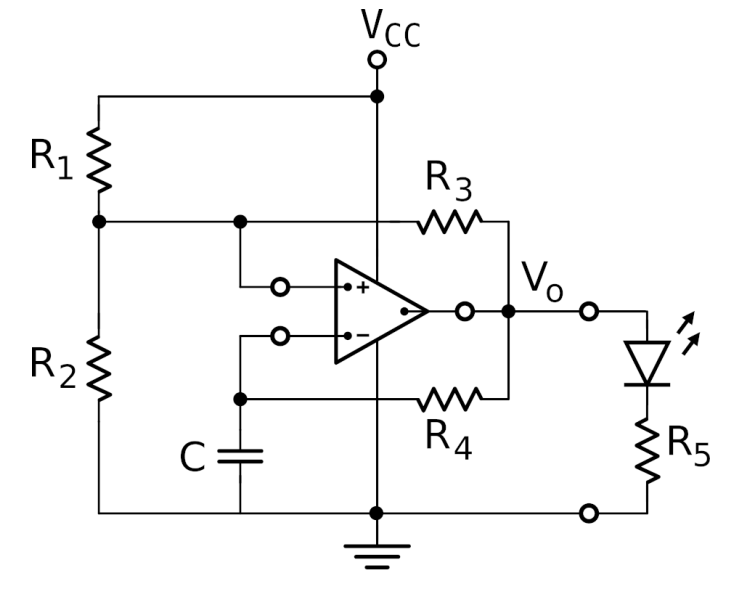
\includegraphics[width=0.5\columnwidth]{images/o_circuito.png}
    \caption{Oscilador astável com LED.}
\end{figure}

\newpage
\subsection{Análise simbólica}

A análise é conduzida, examinando-se combinacao de estados do diodo e do amp op separadamente. O processo tem início com o diodo polarizado diretamente, seguido pelo diodo polarizado reversamente.

\subsubsection{Restrições}

A análise é conduzida ao examinar a combinação de estados do diodo e do amp op separadamente. O processo tem início com o diodo polarizado diretamente, seguido pelo diodo polarizado reversamente.

\begin{equation}
    V_{m1} < V_{D0} < V_{m2}
\end{equation}

Também, quando o LED está polarizado diretamente, tem-se que:

\begin{equation}
    \begin{aligned}
         & I_L > 0      \\
         & V_d = V_{D0}
    \end{aligned}
\end{equation}

Quando o LED está polarizado inversamente:

\begin{equation}
    \begin{aligned}
         & I_L = 0      \\
         & V_d < V_{D0}
    \end{aligned}
\end{equation}

\subsubsection{Estado 1: Amp Op ligado e diodo polarizado diretamente}

\begin{figure}[H]
    \centering
    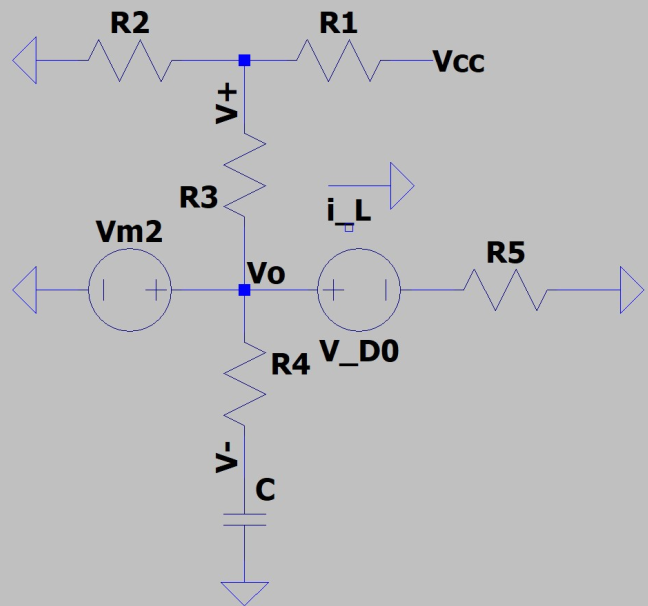
\includegraphics[width=0.5\columnwidth]{images/ampop1diodo1.png}
    \caption{Amp op ligado, diodo polarizado diretamente.}
\end{figure}

Neste estado, ambos LED e amp op estão ligados e tem-se a seguinte análise:

\begin{equation}
    \begin{aligned}
         & \frac{V_{m2} - V_{D0}}{R_5} = I_L \\
         & V_{m2} > V_{D0}                   \\
         & I_L > 0
    \end{aligned}
\end{equation}

Como pode-se observar, a análise não contradiz as restrições, logo este estado é possível.

Entao o analisaremos e resolveremos as equacoes diferenciais que vem dele.

\begin{equation}
    \begin{aligned}
         & \frac{- V_{o} + V_{+}}{R_{3}} + \frac{V_{+}}{R_{2}} + \frac{- VCC + V_{+}}{R_{1}} = 0 \\
         & C \frac{d}{d t} V_{c} + V_{c} - V_{m2} = 0                                            \\
         & V_{o} = V_{m2}                                                                        \\
    \end{aligned}
\end{equation}

Resolvemos a primeira expressão acima isolando $V_{+}$ e a segunda expressão por Laplace isolando o $V_c"$ e obtemos:

\begin{equation}
    \begin{aligned}
         & V_{+} = V_2 = \frac{R_{1} R_{2} V_{m2} + R_{2} R_{3} VCC}{R_{1} R_{2} + R_{1} R_{3} + R_{2} R_{3}} \\
         & V_c = u(t) \left( V_{m2} + (V_{C0} - V_{m2}) e^{\frac{-t}{R_4 C}} \right)                          \\
    \end{aligned}
\end{equation}

Como visto, o $V_c$ se comporta como um circuito $RC$ em resposta forçada. Logo, a nossa constante de tempo é:

\begin{equation}
    \tau = R C = R_4 C
\end{equation}

\subsubsection{Estado 2: Amp Op desligado e diodo polarizado inversamente}

\begin{figure}[H]
    \centering
    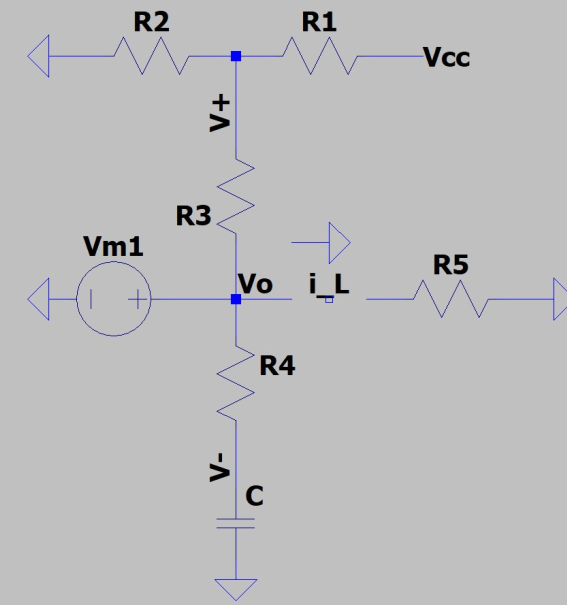
\includegraphics[width=0.5\columnwidth]{images/ampop2diodo2.png}
    \caption{Amp op desligado, diodo polarizado inversamente.}
\end{figure}

Neste estado, ambos LED e amp op estão desligados e tem-se a seguinte análise:

\begin{equation}
    \begin{aligned}
         & \frac{V_{m1} - V_{D0}}{R_5} = I_L \\
         & I_L = 0                           \\
         & V_{m1} = V_{D0}                   \\
         & V_{m1} < V_{D0}                   \\
         & V_D < V_{D0}
    \end{aligned}
\end{equation}

Como pode-se observar, a análise não contradiz as restrições, logo este estado é possível.

Então, o analisaremos e resolveremos as equações diferenciais que vêm dele.

\begin{equation}
    \begin{aligned}
         & \frac{V_{+} - V_{o}}{R_3} +  \frac{V_{+} - VCC}{R_1} + \frac{V_{+}}{R_2} = 0 \\
         & C \frac{d}{d t} V_{c} + V_{c} - V_{m1} = 0                                   \\
         & V_{o} = V_{m1}                                                               \\
    \end{aligned}
\end{equation}

Resolvemos a primeira expressão acima isolando $V_{+}$ e a segunda expressão, por Laplace, isolando o $V_c$, e obtemos:

\begin{equation}
    \begin{aligned}
         & V_{+} = V_1 = \frac{R_{1} R_{2} V_{m1} + R_{2} R_{3} VCC}{R_{1} R_{2} + R_{1} R_{3} + R_{2} R_{3}} \\
         & V_c = u(t) \left( V_{m1} + (V_{C0} - V_{m1}) e^{\frac{-t}{R_4 C}} \right)                          \\
    \end{aligned}
\end{equation}

Como visto, o $V_c$ comporta-se como um circuito $RC$ em resposta forçada, logo a nossa constante de tempo é:

\begin{equation}
    \tau = R C = R_4 C
\end{equation}

\subsubsection{Estado 3: Amp Op ligado e diodo polarizado inversamente}

\begin{figure}[H]
    \centering
    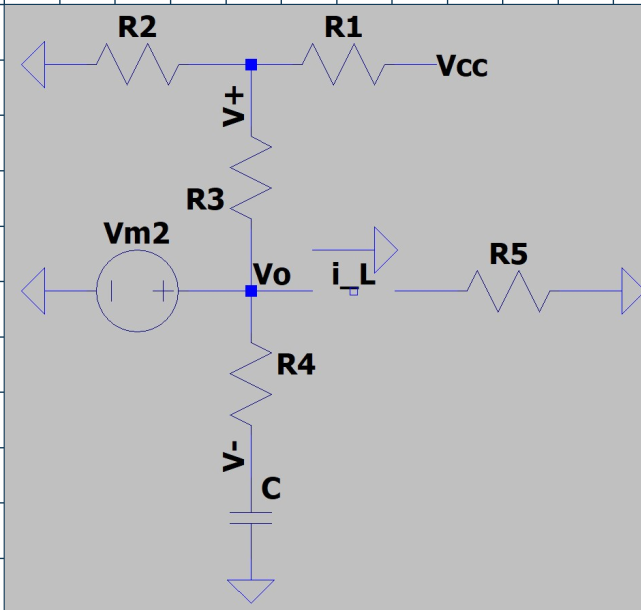
\includegraphics[width=0.5\columnwidth]{images/ampop1diodo2.png}
    \caption{Amp op ligado, diodo polarizado inversamente.}
\end{figure}

Neste estado, o LED está desligado e o amp op está ligado, e tem-se a seguinte análise:

\begin{equation}
    \begin{aligned}
         & \frac{V_{m2} - V_{D}}{R_5} = I_L \\
         & I_L = 0                          \\
         & V_{m2} = V_{D}                   \\
         & V_{m2} > V_{D0}                  \\
         & V_D > V_{D0}
    \end{aligned}
\end{equation}

Como pode-se observar, a análise contradiz a restrição 1, logo este estado é impossível.

\subsubsection{Estado 4: Amp Op desligado e diodo polarizado diretamente}

\begin{figure}[H]
    \centering
    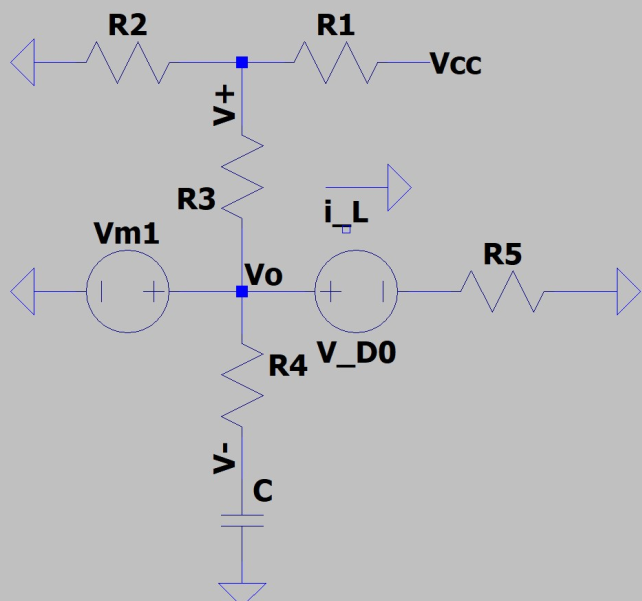
\includegraphics[width=0.5\columnwidth]{images/ampop2diodo1.png}
    \caption{Amp op ligado, diodo polarizado inversamente.}
\end{figure}

Neste estado, o LED está ligado e o amp op está desligado, e tem-se a seguinte análise:

\begin{equation}
    \begin{aligned}
         & \frac{V_{m1} - V_{D}}{R_5} = I_L \\
         & V_{m1} < V_{D0}                  \\
         & I_L < 0                          \\
    \end{aligned}
\end{equation}

Como pode-se observar, a análise contradiz a restrição 2, logo este estado é impossível.

\subsubsection{Parametros A e B}

Utilizaremos as equacoes (6) e (10) onde encontramos $V_1$ e $V_2$, e faremos as substituicoes de $A = e^{\frac{-kT}{\tau}}$ e $B = e^{\frac{-(1-k)T}{\tau}}$.

Fazendo estas substituicoes obtemos:

\begin{equation}
    \begin{aligned}
         & A = \frac{V_2 - V_{m2}}{V_1 - V_{m2}} \\
         & B = \frac{V_1 -V_{m1}}{V_2 - V_{m1}}
    \end{aligned}
\end{equation}

Para obter o $T$ e o $k$ fazemos:

\begin{equation}
    \begin{aligned}
        A B = e^{-\frac{T}{\tau}} => T = - \tau \ln(A B) \\
        \frac{A}{B} = e^{\frac{-kT}{\tau} + T - \frac{-kT}{\tau}} => k = e^{\frac{-2kT}{\tau} + T}
    \end{aligned}
\end{equation}

Com isto podemos resolver numericamente para $T$ e $k$ e obtemos:

\begin{equation}
    \begin{aligned}
         & T = \operatorname{=}\operatorname{-} \log{\left( \frac{\left( \ensuremath{\mathrm{V1}}\operatorname{-}\ensuremath{\mathrm{Vm1}}\right) \, \left( \ensuremath{\mathrm{V2}}\operatorname{-}\ensuremath{\mathrm{Vm2}}\right) }{\left( \ensuremath{\mathrm{V2}}\operatorname{-}\ensuremath{\mathrm{Vm1}}\right) \, \left( \ensuremath{\mathrm{V1}}\operatorname{-}\ensuremath{\mathrm{Vm2}}\right) }\right) } \tau                                                                                                                                                                                          \\
         & k = \frac{\log{\left( \frac{\ensuremath{\mathrm{V2}}\operatorname{-}\ensuremath{\mathrm{Vm2}}}{\ensuremath{\mathrm{V1}}\operatorname{-}\ensuremath{\mathrm{Vm2}}}\right) }\operatorname{-}\log{(b)}}{2 \log{\left( \frac{\left( \ensuremath{\mathrm{V1}}\operatorname{-}\ensuremath{\mathrm{Vm1}}\right) \, \left( \ensuremath{\mathrm{V2}}\operatorname{-}\ensuremath{\mathrm{Vm2}}\right) }{\left( \ensuremath{\mathrm{V2}}\operatorname{-}\ensuremath{\mathrm{Vm1}}\right) \, \left( \ensuremath{\mathrm{V1}}\operatorname{-}\ensuremath{\mathrm{Vm2}}\right) }\right) }}\operatorname{+}\frac{1}{2}
    \end{aligned}
\end{equation}

Para obter $V_1$ e $V_2$ podemos dar solve nas equacoes (14):

\begin{equation}
    \begin{aligned}
         & \ensuremath{\mathrm{V_1}}\operatorname{=}\frac{\ensuremath{\mathrm{V_{m2}}} A B\operatorname{-}\ensuremath{\mathrm{V_{m2}}} B\operatorname{+}\ensuremath{\mathrm{V_{m1}}} B\operatorname{-}\ensuremath{\mathrm{V_{m1}}}}{A B\operatorname{-}1}              \\
         & \ensuremath{\mathrm{V_2}}\operatorname{=}\frac{A\, \left( \ensuremath{\mathrm{V_{m1}}} B\operatorname{+}\ensuremath{\mathrm{V_{m2}}}\operatorname{-}\ensuremath{\mathrm{V_{m1}}}\right) \operatorname{-}\ensuremath{\mathrm{V_{m2}}}}{A B\operatorname{-}1}
    \end{aligned}
\end{equation}

\subsubsection{Resistencias}

Utilizando as equações (6) e (10), podemos resolver $R_1$ e $R_2$.

\begin{equation}
    \begin{aligned}
         & \ensuremath{\mathrm{R1}}\operatorname{=}\operatorname{-}\left( \frac{\ensuremath{\mathrm{R3}}\, \ensuremath{\mathrm{Vcc}}\, \ensuremath{\mathrm{v2}}\operatorname{-}\ensuremath{\mathrm{R3}}\, \ensuremath{\mathrm{Vcc}}\, \ensuremath{\mathrm{v1}}}{\ensuremath{\mathrm{Vm1}}\, \ensuremath{\mathrm{v2}}\operatorname{-}\ensuremath{\mathrm{Vm2}}\, \ensuremath{\mathrm{v1}}}\right)                                                                                                                                                                                                                             \\
         & \ensuremath{\mathrm{R2}}\operatorname{=}\frac{\ensuremath{\mathrm{R3}}\, \ensuremath{\mathrm{Vcc}}\, \ensuremath{\mathrm{v2}}\operatorname{-}\ensuremath{\mathrm{R3}}\, \ensuremath{\mathrm{Vcc}}\, \ensuremath{\mathrm{v1}}}{\left( \ensuremath{\mathrm{Vm1}}\operatorname{-}\ensuremath{\mathrm{Vcc}}\right) \, \ensuremath{\mathrm{v2}}\operatorname{+}\left( \ensuremath{\mathrm{Vcc}}\operatorname{-}\ensuremath{\mathrm{Vm2}}\right) \, \ensuremath{\mathrm{v1}}\operatorname{+}\ensuremath{\mathrm{Vcc}}\, \ensuremath{\mathrm{Vm2}}\operatorname{-}\ensuremath{\mathrm{Vcc}}\, \ensuremath{\mathrm{Vm1}}} \\
    \end{aligned}
\end{equation}

Utilizando (7) obtemos $R_3$:

\begin{equation}
    R_4=\frac{\tau}{C}
\end{equation}

Utilizando (4) obtemos $R_5$:

\begin{equation}
    \ensuremath{\mathrm{R5}}\operatorname{=}\frac{\ensuremath{\mathrm{Vo}}\operatorname{-}\ensuremath{\mathrm{Vd0}}}{\ensuremath{\mathrm{i_L}}}
\end{equation}


\subsection{Projetando o circuito}

Com a análise teórica feita, analisaremos dois exemplos. Em ambos os exemplos, teremos os seguintes parâmetros:

\begin{equation}
    \begin{aligned}
         & V_{CC} = 11 V  \\
         & V_{D0} = 2 V   \\
         & V_{m1} = 0.3 V \\
         & V_{m2} = 9.2 V \\
         & I_L = 12 mA    \\
    \end{aligned}
\end{equation}

\subsubsection{Exemplo 1}

Utilizando os dados acima para o exemplo 1 obtemos:

\begin{equation}
    \begin{aligned}
         & A = 0.7788             \\
         & B = 0.7788             \\
         & V_1 = 4.1966 V         \\
         & V_2 = 5.3034 V         \\
         & R_1 = 15.45k \varOmega \\
         & R_2 = 11.47k \varOmega \\
         & R_3 = 47k \varOmega    \\
         & R_4 = 100k \varOmega   \\
         & R_5 = 600 \varOmega    \\
         & C = 10 \mu F           \\
    \end{aligned}
\end{equation}

\subsubsection{Exemplo 2}

Utilizando os dados acima para o exemplo 2 obtemos:

\begin{equation}
    \begin{aligned}
         & A = 0.2636             \\
         & B = 0.1353             \\
         & V_1 = 1.22 V           \\
         & V_2 = 7.01 V           \\
         & R_1 = 124.9k \varOmega \\
         & R_2 = 47k \varOmega    \\
         & R_3 = 17.6k \varOmega  \\
         & R_4 = 20k \varOmega    \\
         & R_5 = 600 \varOmega    \\
         & C = 100 nF             \\
    \end{aligned}
\end{equation}